\subsection{Gateway}
			\subsubsection{Diagramma delle classi}

		  	\begin{figure}[H]
				\centering
				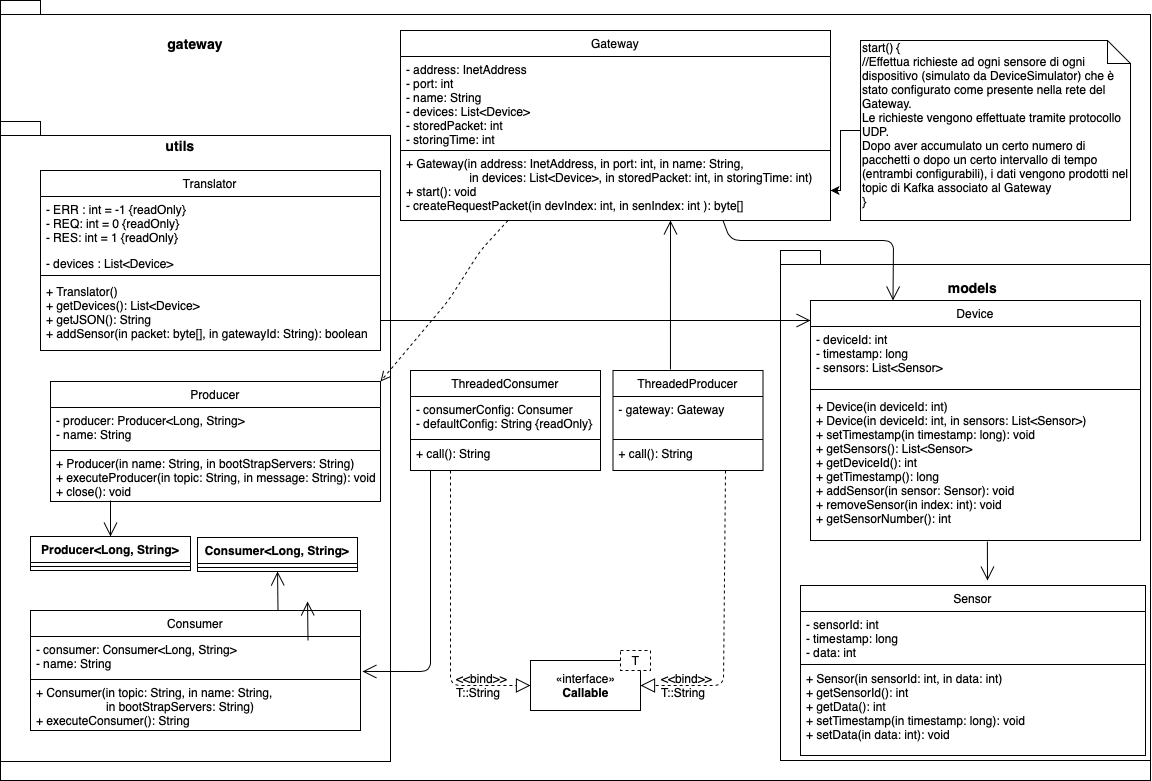
\includegraphics[scale=0.675]{res/images/ClassiGateway.png}
				\caption{Diagramma delle classi per la componente gateway}
			\end{figure}	

			\subsubsection{Diagramma di sequenza}

		  	\begin{figure}[H]
				\centering
				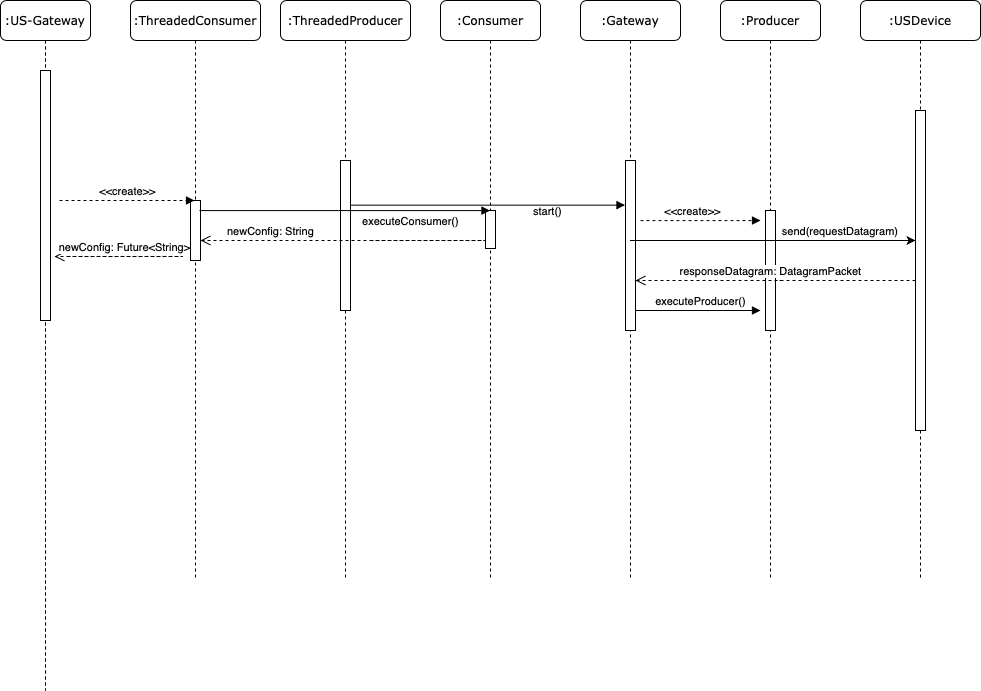
\includegraphics[scale=0.675]{res/images/RichiestaInvioGateway.png}
				\caption{Diagramma di sequenza che rappresenta la richiesta di un dato e il conseguente invio del messaggio a un topic di Kafka}
			\end{figure}

			Nel diagramma precedente sono stati mezionati in minima parte sia il simulatore dispositivi per una questione di continuità che il consumer per mostrare nella sua interezza ciò che avviene all'interno del gateway.








